\documentclass{standalone}
\usepackage{tikz}
\usepackage{circuitikz}
\usetikzlibrary{positioning}

\begin{document}
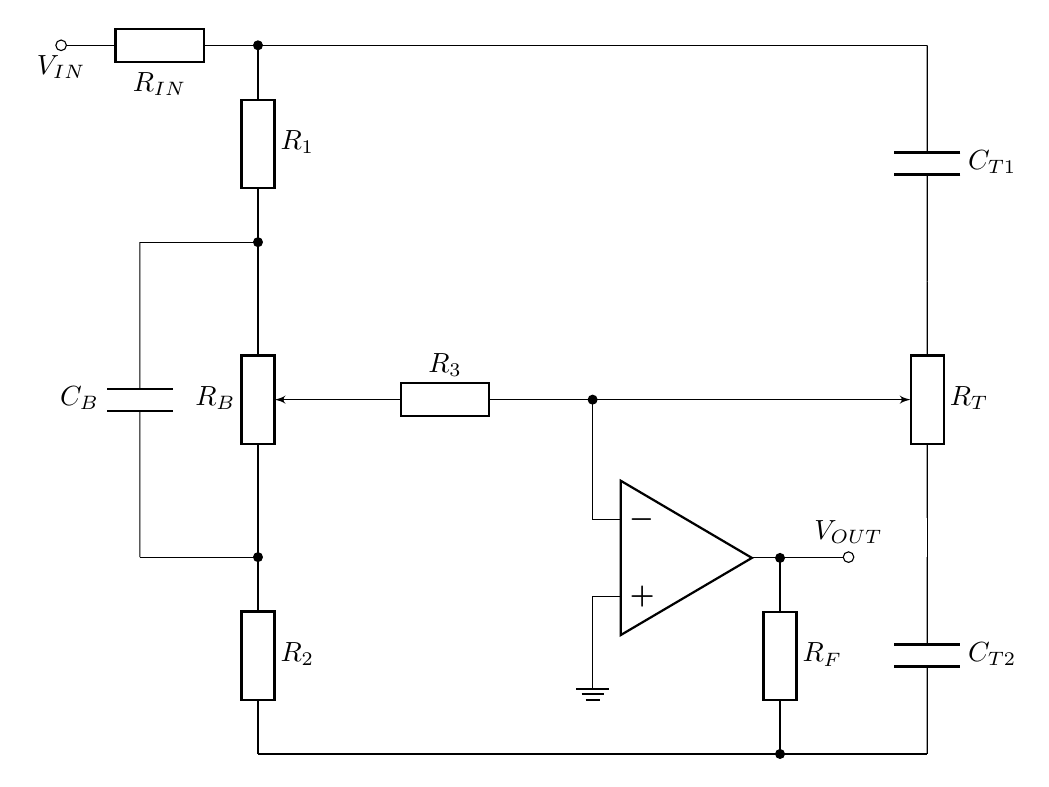
\begin{tikzpicture}
	% Instances/Symbols:
	\node[op amp] at (9.44, 3.49) {};
	\node[ground] at (8.25, 2.25) {};
	
	\draw (4, 10) to[european resistor, l=$R_{IN}$] (1.5, 10);	
	\draw (4, 10) to[european resistor, l=$R_1$] (4, 7.5);
	\draw (4, 3.5) to[european resistor, l=$R_2$] (4, 1);
	\draw (4.5, 5.5) to[european resistor, l=$R_3$] (8.25, 5.5);
	\draw (10.63, 3.49) to[european resistor, l=$R_F$] (10.63, 1);

	\draw (2.5, 7.5) to[capacitor, l_=$C_B$] (2.5, 3.5);
	\draw (12.5, 10) to[capacitor, l=$C_{T1}$] (12.5, 7);
	\draw (12.5, 1) to[capacitor, l_=$C_{T2}$] (12.5, 3.5);
	
	\draw (4, 7.5) to[european potentiometer, l_=$R_B$] (4, 3.5);
	\draw (12.5, 4) to[european potentiometer, l_=$R_T$] (12.5, 7);

	% Lines:
	\draw (2.5, 7.5) -- (4, 7.5);
	\draw (2.5, 3.5) -- (4, 3.5);
	\draw (8.25, 2.25) -- (8.25, 3);
	\draw (8.25, 3.98) -| (8.25, 5.5);
	\draw (11.5, 3.5) |- (10.63, 3.49);
	\draw (4, 10) -- (12.5, 10);
	\draw (12.5, 3.5) -- (12.5, 4);
	\draw (8.25, 5.5) -- (12, 5.5);
	\draw (4, 1) -- (12.5, 1);

	% Nodes:
	\node[circ] at (4, 10) {};
	\node[circ] at (4, 7.5) {};
	\node[circ] at (4, 3.5) {};
	% \node[circ] at (6, 5.5) {};
	\node[circ] at (8.25, 5.5) {};
	\node[circ] at (10.63, 1) {};
	\node[circ] at (10.63, 3.49) {};
	\node[ocirc, scale=1.2] at (1.5, 10) {};
	\node[ocirc, scale=1.2] at (11.5, 3.5) {};

	% Labels
	\node[below=0cm of {1.5, 10}] {$V_{IN}$};
	\node[above=0.05cm of {11.5, 3.5}] {$V_{OUT}$};

\end{tikzpicture}
\end{document}